% !TEX root = ../main.tex
%ex15_fig3.tex
%couronne de taille 10

\begin{figure}[h]
	\begin{center}
		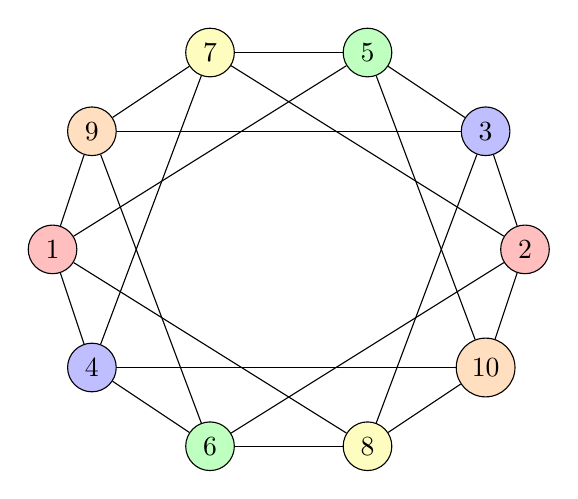
\begin{tikzpicture}
			\tikzset{node/.style={circle, draw=black}};
			\node[node,fill=green!25] (a) at (2,0) {6};
			\node[node,fill=yellow!25] (b) at (4,0) {8};
			\node[node,fill=blue!25] (c) at (0.5,1) {4};
			\node[node,fill=orange!25] (d) at (5.5,1) {10};
			\node[node,fill=red!25] (e) at (0,2.5) {1};
			\node[node,fill=red!25] (f) at (6,2.5) {2};
			\node[node,fill=orange!25] (g) at (0.5,4) {9};
			\node[node,fill=blue!25] (h) at (5.5,4) {3};
			\node[node,fill=yellow!25] (i) at (2,5) {7};
			\node[node,fill=green!25] (j) at (4,5) {5};

			\draw[black] (a) -- (b);
			\draw[black] (b) -- (d);
			\draw[black] (a) -- (c);
			\draw[black] (c) -- (e);
			\draw[black] (d) -- (f);
			\draw[black] (e) -- (g);
			\draw[black] (f) -- (h);
			\draw[black] (g) -- (i);
			\draw[black] (h) -- (j);
			\draw[black] (i) -- (j);
			
			\draw[black] (a) -- (g);
			\draw[black] (a) -- (f);
			\draw[black] (b) -- (h);
			\draw[black] (b) -- (e);
			\draw[black] (c) -- (d);
			\draw[black] (c) -- (i);
			\draw[black] (d) -- (j);
			\draw[black] (e) -- (j);
			\draw[black] (f) -- (i);
			\draw[black] (g) -- (h);
		\end{tikzpicture}
	\end{center}
	\caption{Coloration de la couronne par l'algorithme}
	\label{ex15_fig3}
\end{figure}


